% Relatório do laboratório 5 de servo
% Felipe Bandeira da Silva
% 27/09/2013

%\documentclass[a4paper, 10pt]{article}
\documentclass[paper=a4, fontsize=11pt]{article}

\usepackage[framed,numbered,autolinebreaks,useliterate]{mcode}

\usepackage[brazil]{babel}
\usepackage[utf8]{inputenc}
\usepackage{listings}
\usepackage{color}
\usepackage{amsthm}
\usepackage{graphicx}

\usepackage{schemabloc}
\usetikzlibrary{circuits}

\setlength{\parindent}{0pt}
\setlength{\parskip}{18pt}

\title{Relatório, Laboratório 5.\\Servo 1}
\author{Felipe Bandeira da Silva}
\date{}

%%%%%%%%%%%%%%%%%%%%%%%%%%%%%%%%%%%%%%%%%%%%%%%%%%%%%%%%%%%%%%%%%%%%%%%%%%%%%%%%
% MAIN
%%%%%%%%%%%%%%%%%%%%%%%%%%%%%%%%%%%%%%%%%%%%%%%%%%%%%%%%%%%%%%%%%%%%%%%%%%%%%%%%

\begin{document}


\maketitle

Utilizar o Matlab para analisar a resposta transitória de sistemas de 2ª ordem e 
estudar o efeito do controle proporcional sobre a resposta transitória.

\newpage

\listoffigures

\newpage

%%%%%%%%%%%%%%%%%%%%%%%%%%%%%%%%%%%%%%%%%%%%%%%%%%%%%%%%%%%%%%%%%%%%%%%%%%%%%%%%
% Primeira questão
%%%%%%%%%%%%%%%%%%%%%%%%%%%%%%%%%%%%%%%%%%%%%%%%%%%%%%%%%%%%%%%%%%%%%%%%%%%%%%%%

\section{Efeitos do coeficiente de amortecimento $\zeta$ e a frequência natural
não amortecida $\omega_n$}

Neste problema é necessário analisar a resposta ao degrau para o sistema 
padrão de segunda ordem para as diversas variações de $\zeta$ e $\omega$. 

\subsection{Variação de $\omega_n$}

Para este item $\zeta$ é fixo e de valor 0.4. Mas $\omega_n$ assume os seguintes
valores: 0, 0.4, 0.6, 0.8, 1.0 e 1.4.

A equação padrão para a analise é,

\begin{equation}
    G(s) = \frac{\omega_n^2}{s^2 + 2 \zeta \omega_n s + \omega_n^2}
\end{equation}

Utilizando o seguinte código para facilitar a analise, 

\begin{lstlisting}
zeta = 0.4;
wn = [10 5 1];
t = 0:0.01:10;
cor = ['b', 'g', 'r']
for c = 1:length(wn)
    gs = tf([wn(c)^2], [1 2*zeta*wn(c) wn(c)^2]);
    [y(c,:)] = step(gs, t);
    hold on;
    plot(t, y(c,:), cor(c));
    grid on;
end
xlabel('tempo segundos');
\end{lstlisting}

A figura 1, mostra a resposta para as diversas variações de $\omega_n$

\begin{figure}
    \begin{center}
    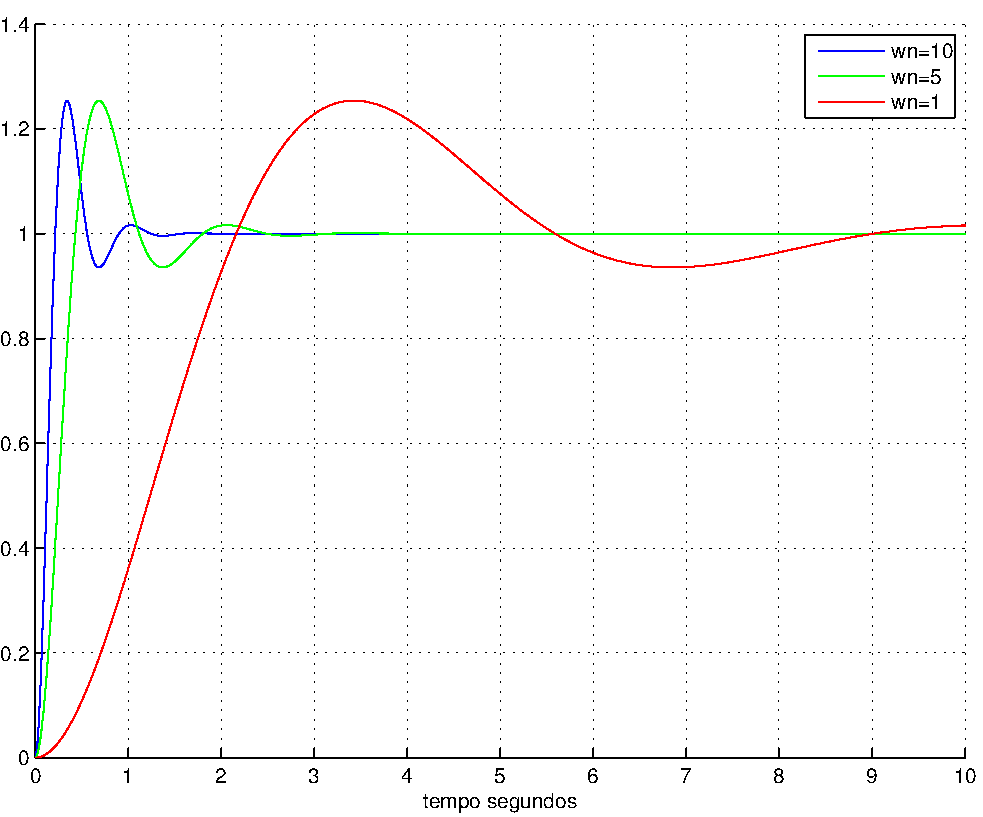
\includegraphics[scale=.5]{q1ia.pdf}
    \caption{Variações de $\omega_w$}
    \end{center}
\end{figure}

\subsection{Variação de $\zeta$}

Neste problema $\omega_n$ é fixo com valor de 5 e $\zeta$ assume os seguintes
valores: 0, 0.4, 0.6, 0.8, 1.0, 1.4.

Para tanto o mesmo código utilizado anteriormente para a analise de $\omega_n$
pode ser alterado para as variações de $\zeta$ de tal forma que fica,

\begin{lstlisting}
zeta = [0 0.4 0.6 0.8 1 1.4];
wn = 5;
t = 0:0.001:4;
cor = ['b', 'g', 'r', 'c', 'm', 'y'];
for c = 1:length(zeta)
    gs = tf([wn^2], [1 2*zeta(c)*wn wn^2]);
    [y(c,:)] = step(gs, t);
    hold on;
    plot(t, y(c,:), cor(c));
    grid on;
end
xlabel('tempo segundos');
\end{lstlisting}

A resposta para as diversas variações de $\zeta$ é apresentada na figura 2,

\begin{figure}
    \begin{center}
    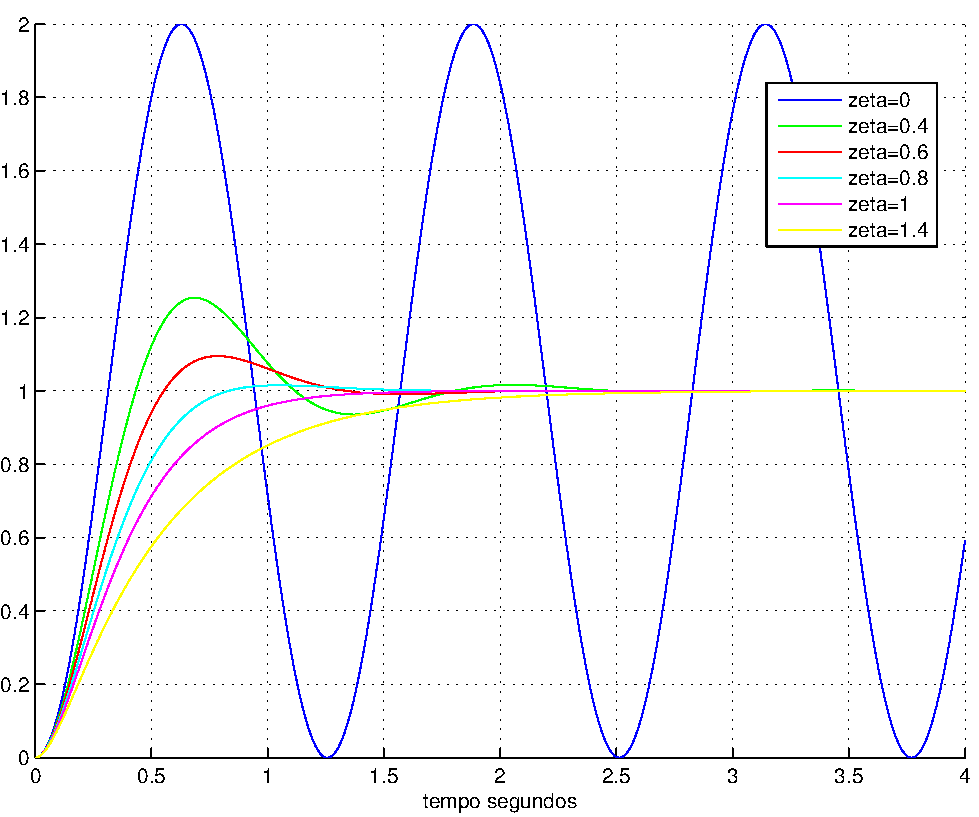
\includegraphics[scale=.5]{q1ib.pdf}
    \caption{Variações de $\zeta$}
    \end{center}
\end{figure}

\subsection{Comentários sobre a variação de $\omega_n$ e $\zeta$}

Como já foi notado os valores de $\omega_n$ e $\zeta$ influenciam no comportamento
de uma função de transferência de segunda ordem. $\omega_n$ está diretamente ligado
a frequência de oscilação do sistema. $\zeta$ está ligada ao tipo de comportamento
do sistema, onde são conhecida as seguintes situações: 

\begin{enumerate}
    \item Sistema subamortecido, quando $0<\zeta<1$
    \item Sistema criticamente amortecido, quando $\zeta = 1$
    \item Sistema superamortecido, quando $\zeta > 1$
    \item Oscilatório, quando $\zeta = 0$
\end{enumerate}

O problema proposta apresenta todas as quatro situações. A analise para
o sistema de segundo ordem pode então ser feita vendo apenas os parâmetros
ou valores de $\omega_n$ e $\zeta$


\section{Visualização 3D das variações de $\zeta$}

O grafico 3 mostra uma visão

\begin{figure}[!h]
    \begin{center}
    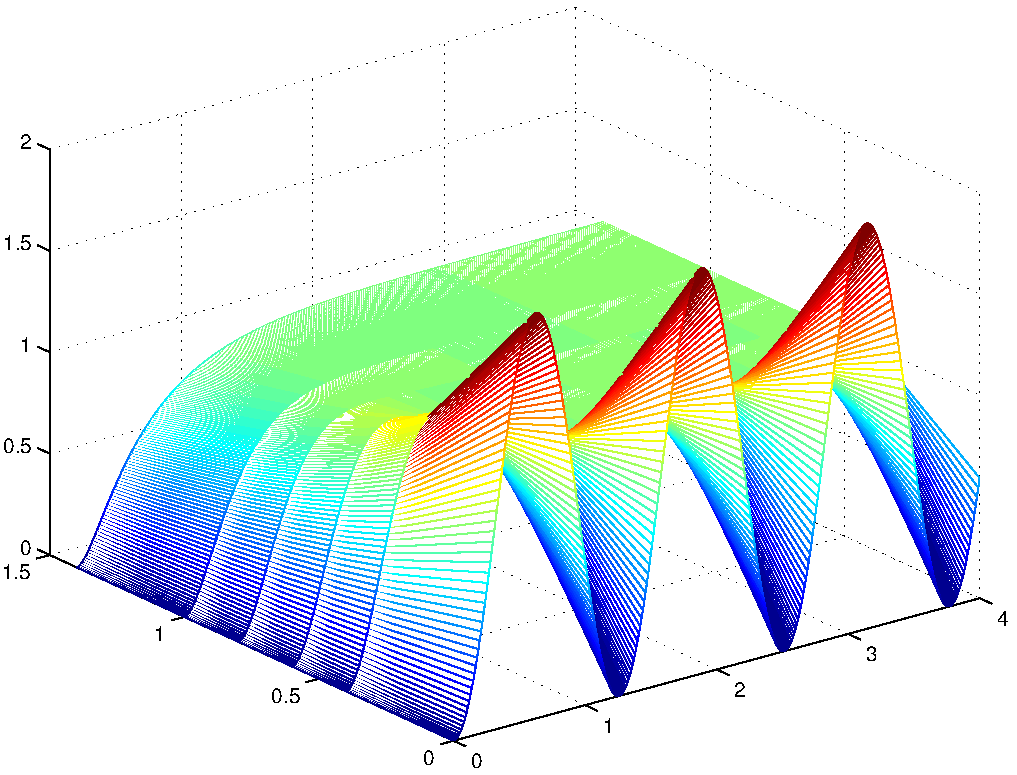
\includegraphics[scale=.5]{q1p2.pdf}
    \caption{Gráfico 3D}
    \end{center}
\end{figure}


\section{Resposta ao impulso}

O sistema proposto é modelado,

\begin{equation}
    \frac{C(s)}{R(s)} = \frac{1}{s^2+s+1}
\end{equation}

A sua resposta para o \textbf(impulso) pode ser encontrada usando as 
seguintes linhas de códigos,

\begin{lstlisting}
gs = tf([1], [1 1 1]);
impulse(gs);
\end{lstlisting}

A resposta para tal é,

\begin{figure}[!h]
    \begin{center}
    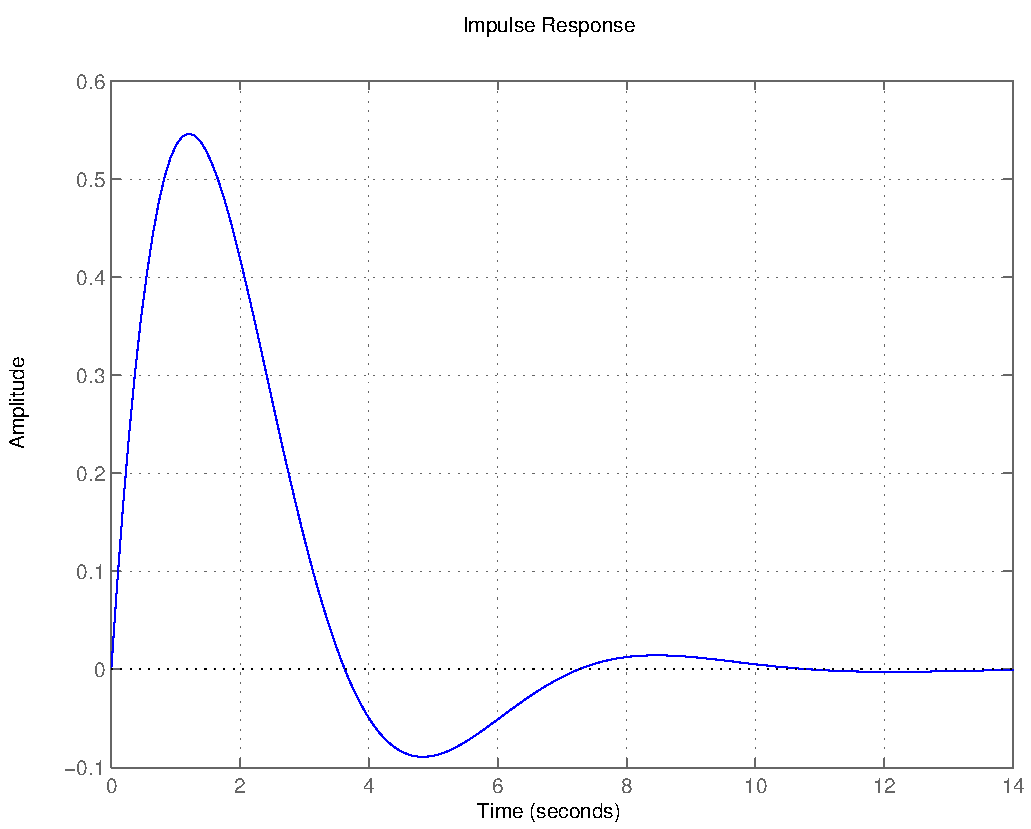
\includegraphics[scale=.5]{q3ia.pdf}
    \caption{Resposta para o impulso de $\frac{1}{s^2+s+1}$}
    \end{center}
\end{figure}


\section{Servo sistema}

Um servosistema possui a seguinte função de transferência,

\begin{equation} \label{eq:servosistema}
    G_p(s) = \frac{z}{J s^2 + B s}
\end{equation}

Onde $J=1 Nm/\frac{rad}{s^2}$ e $B = 4 Nm/\frac{rad}{s}$. Substituindo  os
valores na equação ~\ref{eq:servosistema},

\begin{equation} \label{eq:servosistema}
    G_p(s) = \frac{1}{s^2 + 4 s}
\end{equation}

O sistema finalmente é caracterizado pelo seguinte diagrama de blocos,

\begin{center}
\begin{tikzpicture}
    \sbEntree{E} % entrada
    \sbComp{a}{E} % comparador
    \sbBloc{b}{$K$}{a} % ganho K
        \sbRelier[R(s)]{E}{a} % ligação entrada - comparador
        \sbRelier{a}{b} % ligação comparador - bloco de ganho
    \sbBloc{c}{$\frac{1}{s^2 + 4 s}$}{b} % função de transferência
        \sbRelier{b}{c} % ligação bloco de ganho - função de transferência
    \sbSortie{S}{c}
    \sbRelier{c}{S}
    \sbRenvoi{c-S}{a}{}
    \sbNomLien[.8]{S}{$S_1(s)$}
\end{tikzpicture}
\end{center}

A função de transferência de malha fechada do sistema fica,

\begin{equation}
    \frac{R(s)}{C(s)} = \frac{K G_p(s)}{1 + G_p(s)} = \frac{K}{s^2 + 4 s + 1}
\end{equation}

\subsection{Resposta transitória ao degrau unitario}

Para a resposta transitória faço $K$ varia: 1, 4, 6, 10, 25 e 400. Para tanto
posso utilizar a mesmo código da primeira questão com pequenas modificações, ficando,

\begin{lstlisting}
K = [1 4 6 10 25 400];
t = 0:0.01:40;
cor = ['b', 'g', 'r', 'c', 'm', 'k'];
for c = 1:length(K)
    gs = tf([K(c)], [1 4 K(c)]);
    [y(c,:)] = step(gs, t);
    hold on;
    plot(t, y(c,:), cor(c));
    grid on;
end
xlabel('tempo segundos');
\end{lstlisting}


\begin{figure}
    \begin{center}
    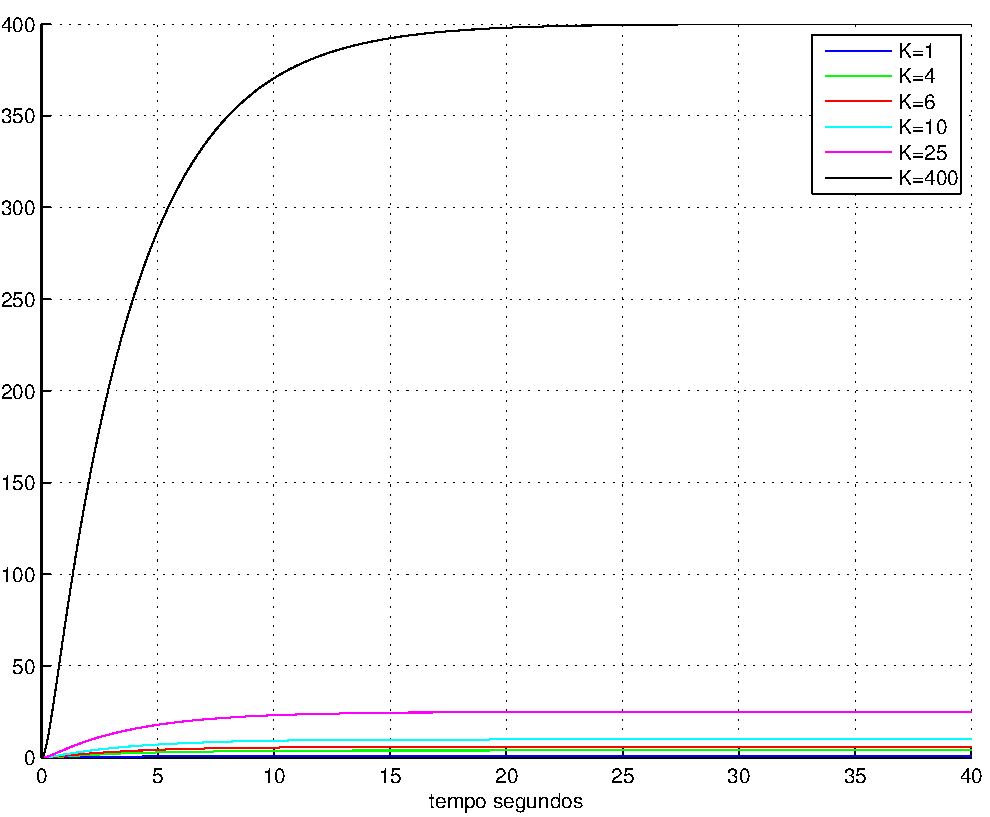
\includegraphics[scale=.5]{q4ia.pdf}
    \caption{Variações de $K$}
    \end{center}
\end{figure}

A figura 4 mostra as diversas resposta para as diversas variações
de $K$, nota-se inicialmente que o erro relativo está diretamente ligado 
a ganho $K$. Com isto é possível concluir que $K$ está ligado as seguintes 
situação, o erro estacionário e resposta do sistema são diretamente proporcionais
a $K$. Agora $K$ não está ligado ao tipo de resposta do sistema, seja ela 
subamortecida, superamortecida, criticamente amortecida ou oscilatória. Esse
tipo de resposta só pode ser modificado com a alteração dos pólos e suas posições
no plano-s. Modificação que deve ser feita na equação característica da função 
de transferência. 

\section{Considerações finais}

Um sistema de segunda ordem difere dos de primeira, pelo fato de possuírem dois polos
mais o fator mais consideravel é o arranjo que este polos estão no plano-s. 
Arranjo este que determina as 4 situações possíveis de resposta para o sistema, 
situações estas que pode ser ou não bem vindas para os componentes do sistema, 
sendo que suas alterações dependem de diversos fatores,  com isto as correções 
para o sistemas de segunda ordem são mais complexas e exigem
um domínio das ferramentas de analise matemática do problema. O Matlab novamente
se mostra um ótimo software para este trabalho matemático, facilitando a visualização
no domínio do tempo das diversas respostas e com simples modificações é possível
criar gráficos complexos.



\end{document}

